\documentclass[11pt,a4paper]{report}
\usepackage[textwidth=37em,vmargin=30mm]{geometry}
\usepackage{calc,xunicode,amsmath,amssymb,paralist,enumitem,tabu,booktabs,datetime2,xeCJK,xeCJKfntef,listings}
\usepackage{tocloft,fancyhdr,tcolorbox,xcolor,graphicx,eso-pic,xltxtra,xelatexemoji}

\newcommand{\envyear}[0]{2024}
\newcommand{\envdatestr}[0]{2024-10-29}
\newcommand{\envfinaldir}[0]{webdb/2024/20241029/final}

\usepackage[hidelinks]{hyperref}
\hypersetup{
    colorlinks=false,
    pdfpagemode=FullScreen,
    pdftitle={Web Digest - \envdatestr}
}

\setlength{\cftbeforechapskip}{10pt}
\renewcommand{\cftchapfont}{\rmfamily\bfseries\large\raggedright}
\setlength{\cftbeforesecskip}{2pt}
\renewcommand{\cftsecfont}{\sffamily\small\raggedright}

\setdefaultleftmargin{2em}{2em}{1em}{1em}{1em}{1em}

\usepackage{xeCJK,xeCJKfntef}
\xeCJKsetup{PunctStyle=plain,RubberPunctSkip=false,CJKglue=\strut\hskip 0pt plus 0.1em minus 0.05em,CJKecglue=\strut\hskip 0.22em plus 0.2em}
\XeTeXlinebreaklocale "zh"
\XeTeXlinebreakskip = 0pt


\setmainfont{Brygada 1918}
\setromanfont{Brygada 1918}
\setsansfont{IBM Plex Sans}
\setmonofont{JetBrains Mono NL}
\setCJKmainfont{Noto Serif CJK SC}
\setCJKromanfont{Noto Serif CJK SC}
\setCJKsansfont{Noto Sans CJK SC}
\setCJKmonofont{Noto Sans CJK SC}

\setlength{\parindent}{0pt}
\setlength{\parskip}{8pt}
\linespread{1.15}

\lstset{
	basicstyle=\ttfamily\footnotesize,
	numbersep=5pt,
	backgroundcolor=\color{black!5},
	showspaces=false,
	showstringspaces=false,
	showtabs=false,
	tabsize=2,
	captionpos=b,
	breaklines=true,
	breakatwhitespace=true,
	breakautoindent=true,
	linewidth=\textwidth
}






\newcommand{\coverpic}[2]{
    % argv: itemurl, authorname
    Cover photo by #2~~(\href{#1}{#1})
}
\newcommand{\makeheader}[0]{
    \begin{titlepage}
        % \newgeometry{hmargin=15mm,tmargin=21mm,bmargin=12mm}
        \begin{center}
            
            \rmfamily\scshape
            \fontspec{BaskervilleF}
            \fontspec{Old Standard}
            \fontsize{59pt}{70pt}\selectfont
            WEB\hfill DIGEST
            
            \vfill
            % \vskip 30pt
            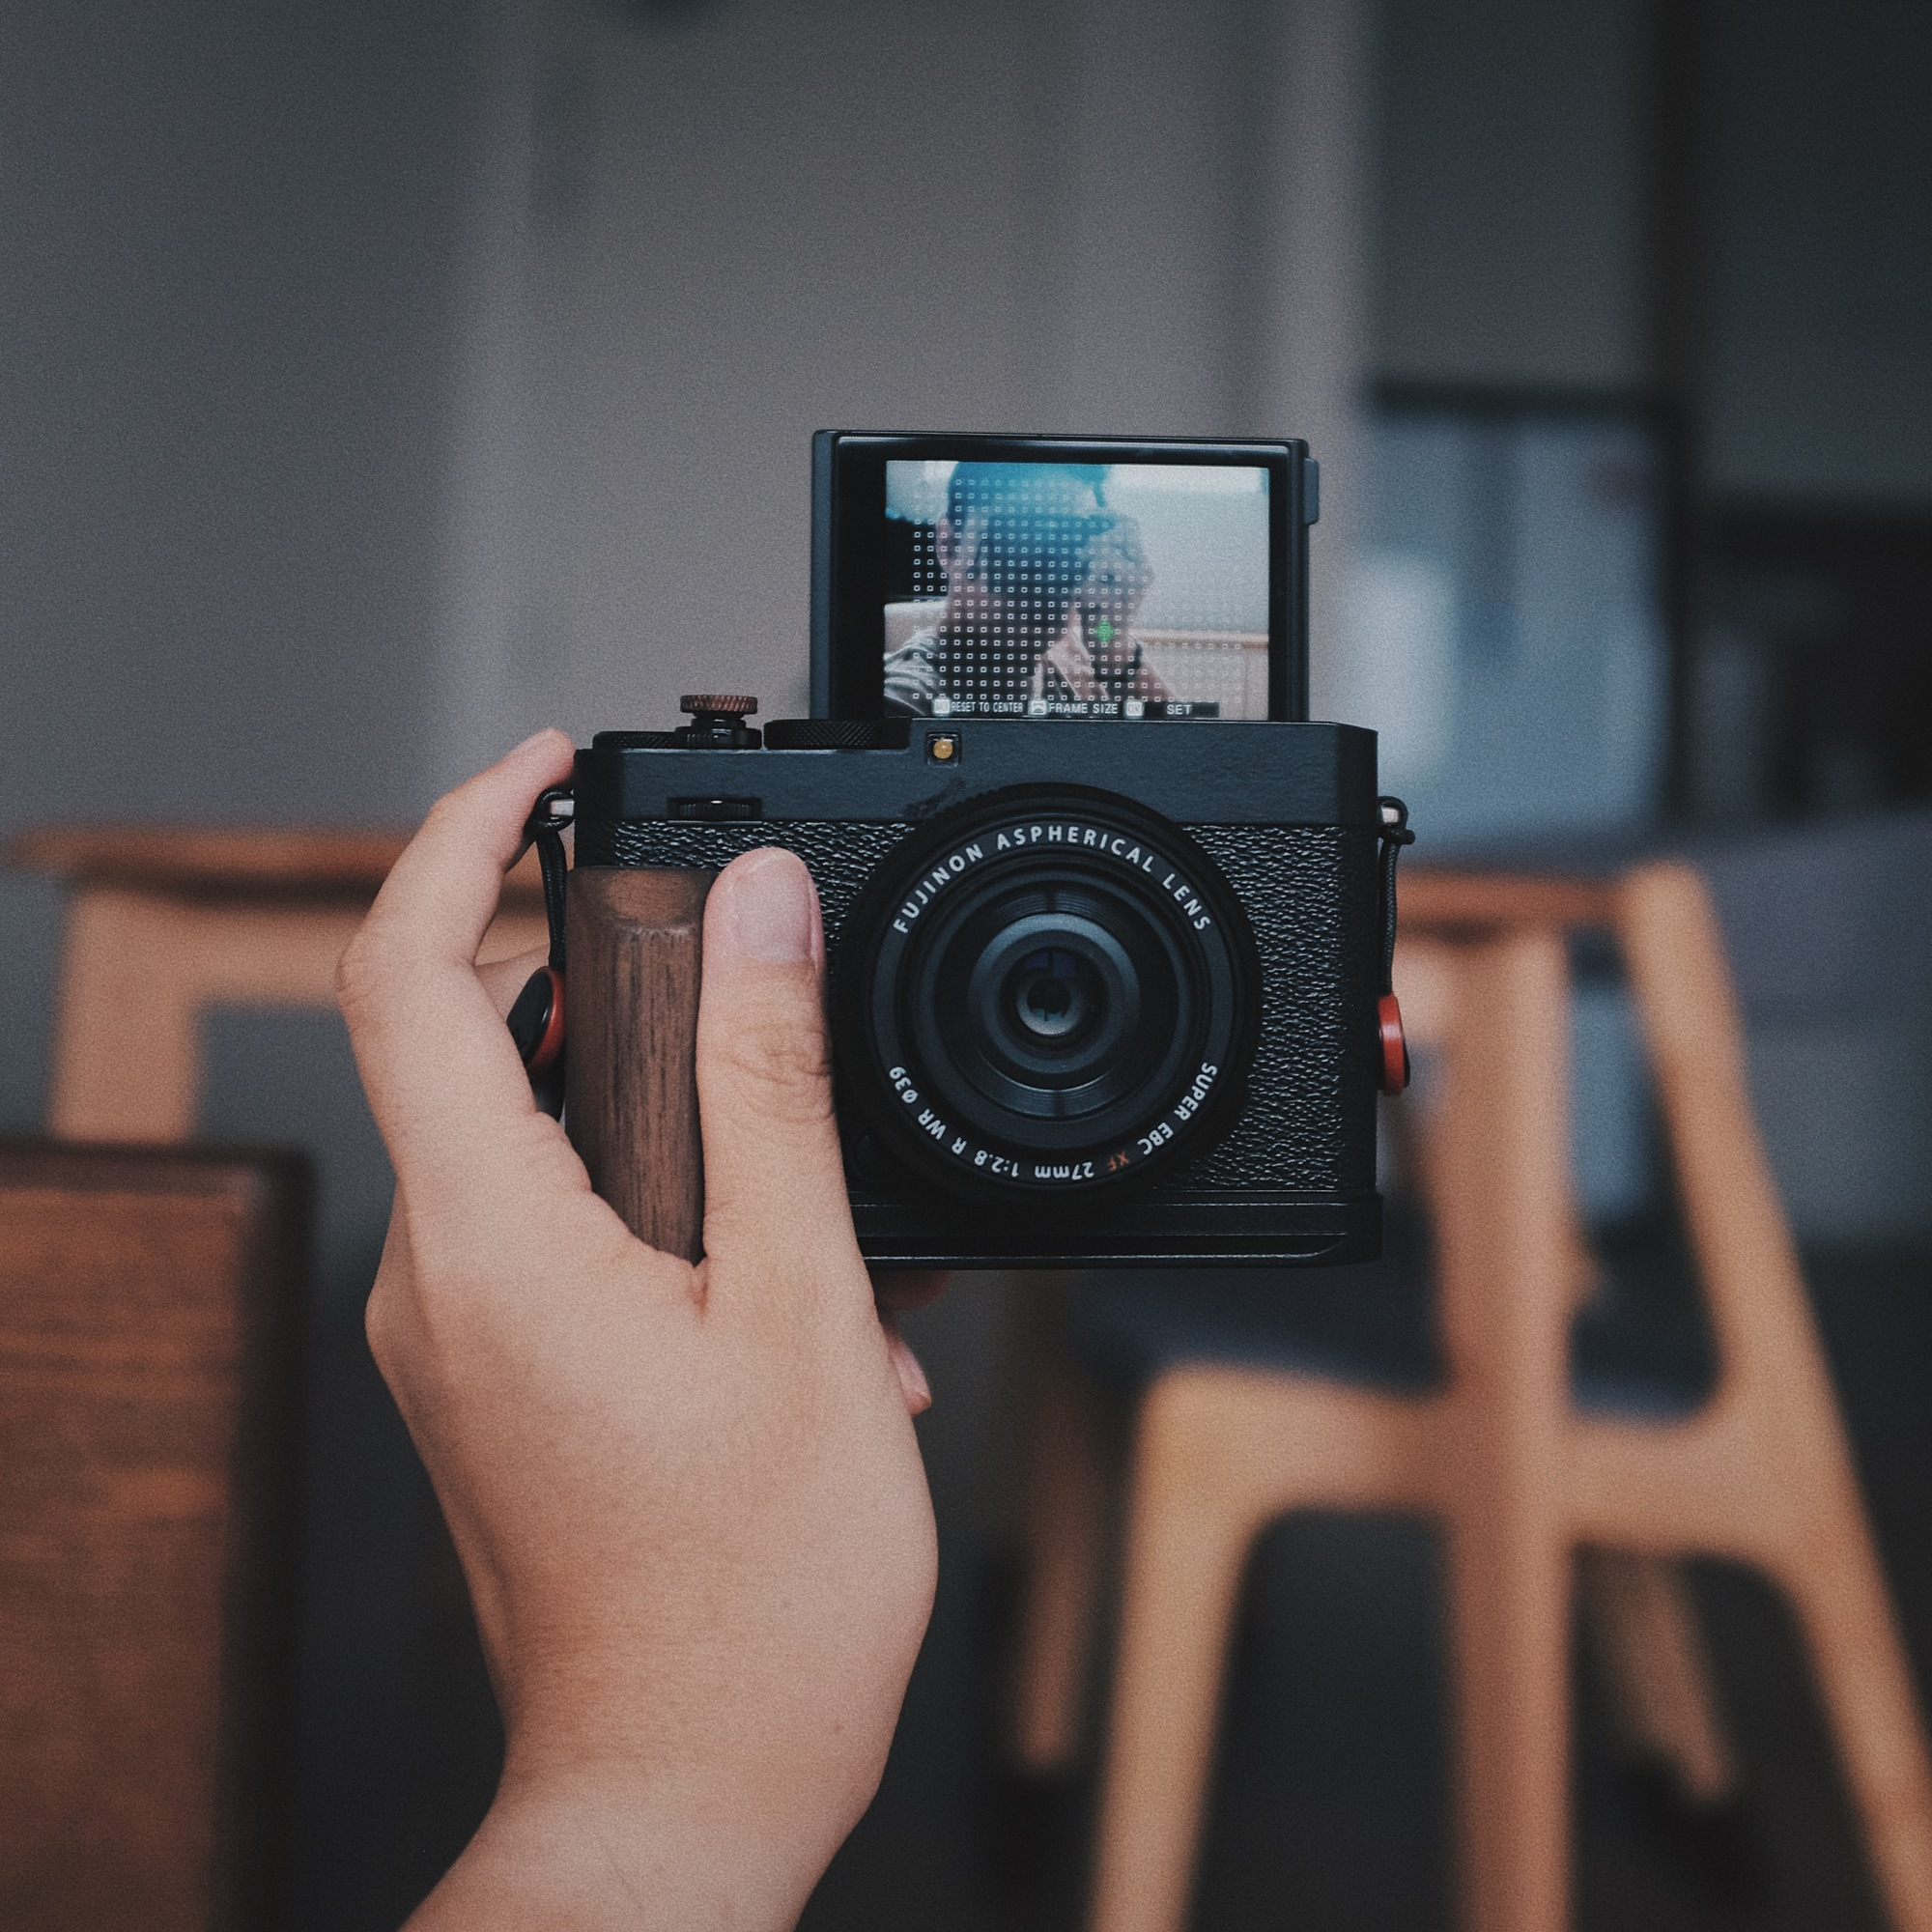
\includegraphics[width=\linewidth]{\envfinaldir/coverpic-prod.jpg}\par
            % \vskip 30pt
            \vfill

            \normalsize\rmfamily\scshape
            \copyright{} The Web Digest Project \hfill\large \envdatestr
        \end{center}
    \end{titlepage}
    % \restoregeometry
}
\newcommand{\simplehref}[1]{%
    \textcolor{blue!80!green}{\href{#1}{#1}}%
}
\renewcommand{\contentsname}{\center\Huge\sffamily\bfseries Contents\par\vskip 20pt}
\newcounter{ipartcounter}
\setcounter{ipartcounter}{0}
\newcommand{\ipart}[1]{
    % \vskip 20pt
    \clearpage
    \stepcounter{ipartcounter}
    \phantomsection
    \addcontentsline{toc}{chapter}{#1}
    % \begin{center}
    %     \Huge
    %     \sffamily\bfseries
    %     #1
    % \end{center}
    % \vskip 20pt plus 7pt
}
\newcounter{ichaptercounter}
\setcounter{ichaptercounter}{0}
\newcommand{\ichapter}[1]{
    % \vskip 20pt
    \clearpage
    \stepcounter{ichaptercounter}
    \phantomsection
    \addcontentsline{toc}{section}{\numberline{\arabic{ichaptercounter}}#1}
    \begin{center}
        \Huge
        \sffamily\bfseries
        #1
    \end{center}
    \vskip 20pt plus 7pt
}
\newcommand{\entrytitlefont}[1]{\subsection*{\raggedright\Large\sffamily\bfseries#1}}
\newcommand{\entryitemGeneric}[2]{
    % argv: title, url
    \parbox{\linewidth}{
        \entrytitlefont{#1}\par\vskip 5pt
        \footnotesize\ttfamily\mdseries
        \simplehref{#2}
    }\vskip 11pt plus 11pt minus 1pt
}
\newcommand{\entryitemGithub}[3]{
    % argv: title, url, desc
    \parbox{\linewidth}{
        \entrytitlefont{#1}\par\vskip 5pt
        \footnotesize\ttfamily\mdseries
        \simplehref{#2}\par\vskip 5pt
        \small\rmfamily\mdseries#3
    }\vskip 11pt plus 11pt minus 1pt
}
\newcommand{\entryitemAp}[3]{
    % argv: title, url, desc
    \parbox{\linewidth}{
        \entrytitlefont{#1}\par\vskip 5pt
        \footnotesize\ttfamily\mdseries
        \simplehref{#2}\par\vskip 5pt
        \small\rmfamily\mdseries#3
    }\vskip 11pt plus 11pt minus 1pt
}
\newcommand{\entryitemHackernews}[3]{
    % argv: title, hnurl, rawurl
    % \parbox{\linewidth}{
    %     \entrytitlefont{#1}\par\vskip 5pt
    %     \footnotesize\ttfamily\mdseries
    %     \simplehref{#3}\par
    %     \textcolor{black!50}{\href{#2}{#2}}
    % }\vskip 11pt plus 11pt minus 1pt
    \begin{minipage}{\linewidth}
            \entrytitlefont{#1}\par\vskip 5pt
            \footnotesize\ttfamily\mdseries
            \simplehref{#3}\par
            \textcolor{black!50}{\href{#2}{#2}}
    \end{minipage}\par\vskip 11pt plus 11pt minus 1pt
}







\begin{document}

\makeheader

\tableofcontents\clearpage




\ipart{Developers}
\ichapter{Hacker News}
\entryitemTwoLinks{A return to hand-written notes by learning to read and write}{https://news.ycombinator.com/item?id=41976311}{https://research.google/blog/a-return-to-hand-written-notes-by-learning-to-read-write/}

\entryitemTwoLinks{200k subscribers flee 'Washington Post' after Bezos blocks Harris endorsement}{https://news.ycombinator.com/item?id=41975395}{https://www.npr.org/2024/10/28/nx-s1-5168416/washington-post-bezos-endorsement-president-cancellations-resignations}

\entryitemTwoLinks{We're forking Flutter}{https://news.ycombinator.com/item?id=41975047}{https://flutterfoundation.dev/blog/posts/we-are-forking-flutter-this-is-why/}

\entryitemTwoLinks{Standardizing Automotive Connectivity}{https://news.ycombinator.com/item?id=41974882}{https://www.tesla.com/en\_CA/blog/standardizing-automotive-connectivity}

\entryitemTwoLinks{So long WordPress}{https://news.ycombinator.com/item?id=41974637}{https://chriswiegman.com/2024/10/so-long-wordpress/}

\entryitemTwoLinks{NY Times gets 230 wrong again}{https://news.ycombinator.com/item?id=41973732}{https://www.techdirt.com/2024/10/28/ny-times-gets-230-wrong-again-misrepresenting-history-law-and-the-first-amendment/}

\entryitemTwoLinks{Using reinforcement learning and \$4.80 of GPU time to find the best HN post}{https://news.ycombinator.com/item?id=41973591}{https://openpipe.ai/blog/hacker-news-rlhf-part-1}

\entryitemTwoLinks{Buy payphones and retire}{https://news.ycombinator.com/item?id=41973065}{https://computer.rip/2024-10-26-buy-payphones-and-retire.html}

\entryitemTwoLinks{The sins of the 90s: Questioning a puzzling claim about mass surveillance}{https://news.ycombinator.com/item?id=41972172}{https://blog.cr.yp.to/20241028-surveillance.html}

\entryitemTwoLinks{New iMac with M4}{https://news.ycombinator.com/item?id=41971726}{https://www.apple.com/newsroom/2024/10/apple-introduces-new-imac-supercharged-by-m4-and-apple-intelligence/}

\entryitemTwoLinks{How Gothic architecture became spooky}{https://news.ycombinator.com/item?id=41969753}{https://www.architecturaldigest.com/story/how-gothic-architecture-became-spooky}

\entryitemTwoLinks{On Good Software Engineers}{https://news.ycombinator.com/item?id=41968892}{https://candost.blog/on-good-software-engineers/}

\entryitemTwoLinks{Write code that is easy to delete, not easy to extend (2016)}{https://news.ycombinator.com/item?id=41968409}{https://programmingisterrible.com/post/139222674273/write-code-that-is-easy-to-delete-not-easy-to}

\entryitemTwoLinks{418 I'm a teapot}{https://news.ycombinator.com/item?id=41967897}{https://developer.mozilla.org/en-US/docs/Web/HTTP/Status/418}

\entryitemTwoLinks{Mill: A fast JVM build tool for Java and Scala}{https://news.ycombinator.com/item?id=41967734}{https://mill-build.org/}

\entryitemTwoLinks{ATL: A layer to run Android apps on Linux}{https://news.ycombinator.com/item?id=41966785}{https://gitlab.com/android\_translation\_layer/android\_translation\_layer/-/blob/master/README.md}

\entryitemTwoLinks{Ask HN: What Are You Working On? (October 2024)}{https://news.ycombinator.com/item?id=41966114}{https://news.ycombinator.com/item?id=41966114}

\entryitemTwoLinks{Platform Strategy and Its Discontents}{https://news.ycombinator.com/item?id=41965091}{https://infrequently.org/2024/10/platforms-are-competitions/}

\entryitemTwoLinks{NotebookLlama: An open source version of NotebookLM}{https://news.ycombinator.com/item?id=41964980}{https://github.com/meta-llama/llama-recipes/tree/main/recipes/quickstart/NotebookLlama}

\entryitemTwoLinks{RP FLIP escapes wrecker's claws}{https://news.ycombinator.com/item?id=41964882}{https://gcaptain.com/saving-rv-flip-from-the-wreckers-clawsand-its-story-is-mind-blowing/}\ichapter{Phoronix}
\entryitemGeneric{\hskip 0pt{}Intel Core Ultra 9 285K Linux Memory DDR5 Performance Testing}{https://www.phoronix.com/review/intel-arrow-lake-ddr5}

\entryitemGeneric{\hskip 0pt{}PCIe TPH Coming With Linux 6.13 To Further Enhance 5th Gen AMD EPYC Performance}{https://www.phoronix.com/news/PCIe-TPH-For-Linux-6.13}

\entryitemGeneric{\hskip 0pt{}Firefox 132 Ready With Certificate Compression, Accelerated SVG Filter Primitives}{https://www.phoronix.com/news/Mozilla-Firefox-132}

\entryitemGeneric{\hskip 0pt{}Trinity TDE R14.1.3 Lets Linux Users Still Enjoy The KDE 3.5 Desktop Experience}{https://www.phoronix.com/news/Trinity-TDE-R14.1.3-KDE3}

\entryitemGeneric{\hskip 0pt{}Sched\_ext Scheduler Idle Selection Being Extended For LLC \& NUMA Awareness}{https://www.phoronix.com/news/sched\_ext-NUMA-Awareness}

\entryitemGeneric{\hskip 0pt{}Qualcomm Adreno Rusticl-Based OpenCL Merged For Mesa 24.3}{https://www.phoronix.com/news/Freedreno-Rusticl-Mesa-24.3}

\entryitemGeneric{\hskip 0pt{}Raspberry Pi OS Now Using Wayland By Default On All Models}{https://www.phoronix.com/news/Raspberry-Pi-OS-Wayland-Default}

\entryitemGeneric{\hskip 0pt{}Intel Preps Linux Driver For Upgraded Display Capabilities With New Hardware}{https://www.phoronix.com/news/Intel-Battlmage-More-Res}

\entryitemGeneric{\hskip 0pt{}AMD STB Support Extended To Latest Ryzen 9000 Series Desktop CPUs}{https://www.phoronix.com/news/AMD-STB-For-Desktop-Ryzen}


\ipart{Developers~~~~(zh-Hans)}
\ichapter{Solidot}
\entryitemGeneric{\hskip 0pt{}Instagram 和 Meta 会降低低观看量视频的质量 }{https://www.solidot.org/story?sid=79610}

\entryitemGeneric{\hskip 0pt{}开源本身不是科技巨头服务的替代}{https://www.solidot.org/story?sid=79609}

\entryitemGeneric{\hskip 0pt{}韦伯望远镜发现了流浪类星体}{https://www.solidot.org/story?sid=79608}

\entryitemGeneric{\hskip 0pt{}昆虫因人为环境变化而改变颜色}{https://www.solidot.org/story?sid=79607}

\entryitemGeneric{\hskip 0pt{}Gentoo 引入了 DTrace}{https://www.solidot.org/story?sid=79606}

\entryitemGeneric{\hskip 0pt{}欧洲犯罪组织天天炸 ATM}{https://www.solidot.org/story?sid=79605}

\entryitemGeneric{\hskip 0pt{}英伟达市值超过苹果}{https://www.solidot.org/story?sid=79604}

\entryitemGeneric{\hskip 0pt{}埃及博主在释放日之后仍然被关押}{https://www.solidot.org/story?sid=79603}

\entryitemGeneric{\hskip 0pt{}新加坡将通过海底电缆从澳大利亚进口太阳能}{https://www.solidot.org/story?sid=79602}

\entryitemGeneric{\hskip 0pt{}NASA 研发能从轨道降落的火星直升机}{https://www.solidot.org/story?sid=79601}

\entryitemGeneric{\hskip 0pt{}OnlyFans 支付给歌手的钱超过了 Spotify}{https://www.solidot.org/story?sid=79600}

\entryitemGeneric{\hskip 0pt{}天文学家在星际空间发现复杂碳分子}{https://www.solidot.org/story?sid=79599}

\entryitemGeneric{\hskip 0pt{}达美航空正式对 CrowdStrike 提起诉讼}{https://www.solidot.org/story?sid=79598}

\entryitemGeneric{\hskip 0pt{}波音探索出售其太空业务}{https://www.solidot.org/story?sid=79597}

\entryitemGeneric{\hskip 0pt{}Google DeepMind 构建 AI 帮助逆转政治极化}{https://www.solidot.org/story?sid=79596}\ichapter{V2EX}
\entryitemGeneric{\hskip 0pt{}[Apple] Apple Intelligence 太无聊了}{https://www.v2ex.com/t/1084462}

\entryitemGeneric{\hskip 0pt{}[Android] 听说小米港版支持双实体 sim+esim,想问一下能下载小米应用商店来安装国内的银行 app 吗?}{https://www.v2ex.com/t/1084461}

\entryitemGeneric{\hskip 0pt{}[VXNA] 申请收录:一派胡言}{https://www.v2ex.com/t/1084460}

\entryitemGeneric{\hskip 0pt{}[YouTube] 是不是最近 Youtube 网页版加强了对未登录用户的观看限制?}{https://www.v2ex.com/t/1084458}

\entryitemGeneric{\hskip 0pt{}[宽带症候群] 求推荐 CCNP/CCIE 学习用的经典实验拓扑}{https://www.v2ex.com/t/1084457}

\entryitemGeneric{\hskip 0pt{}[RSS] [Follow] 丨 50+垂类精选列表}{https://www.v2ex.com/t/1084456}

\entryitemGeneric{\hskip 0pt{}[iOS] shadowrocket 经常有连接错误}{https://www.v2ex.com/t/1084455}

\entryitemGeneric{\hskip 0pt{}[硬件] 装了新机, 分享个目前这个时间点的装机方案, 游戏和办公通吃型}{https://www.v2ex.com/t/1084454}

\entryitemGeneric{\hskip 0pt{}[买买买] 2024 双十一电视决赛圈}{https://www.v2ex.com/t/1084453}

\entryitemGeneric{\hskip 0pt{}[Apple] 新款妙控鼠标不知道有没有升级回报率}{https://www.v2ex.com/t/1084452}

\entryitemGeneric{\hskip 0pt{}[职场话题] 面试圣经}{https://www.v2ex.com/t/1084451}

\entryitemGeneric{\hskip 0pt{}[iPhone] iOS18.1 给``相册''加了需要面容解锁才可打开,重启 iPhone 后就失效了?}{https://www.v2ex.com/t/1084450}

\entryitemGeneric{\hskip 0pt{}[iPhone] 准备 iOS 转鸿蒙-杂谈}{https://www.v2ex.com/t/1084449}

\entryitemGeneric{\hskip 0pt{}[Chrome] Chrome 更新了规范,一堆扩展已停用}{https://www.v2ex.com/t/1084448}

\entryitemGeneric{\hskip 0pt{}[酷工作] [远程办公全职] top5 币圈交易所 150+岗位内推,待遇匹配大厂}{https://www.v2ex.com/t/1084447}

\entryitemGeneric{\hskip 0pt{}[程序员] 国内有哪家公司用 NodeJS 比较多的嘛?或者组?}{https://www.v2ex.com/t/1084446}

\entryitemGeneric{\hskip 0pt{}[MacBook Pro] iMac 发布了, 11 月 8 日开售}{https://www.v2ex.com/t/1084445}

\entryitemGeneric{\hskip 0pt{}[钓鱼] 有信佛的朋友叫我戒掉钓鱼,说会给鱼造成痛苦}{https://www.v2ex.com/t/1084443}

\entryitemGeneric{\hskip 0pt{}[macOS] 妙控板,键盘,键盘全部进入 USB-C 时代}{https://www.v2ex.com/t/1084442}

\entryitemGeneric{\hskip 0pt{}[问与答] 交个补办的白本《劳动手册》给新公司 HR,问题大不大?}{https://www.v2ex.com/t/1084441}

\entryitemGeneric{\hskip 0pt{}[酷工作] [杭州] AI 初创公司 900/天 招前端(1)、后端实习生(1)}{https://www.v2ex.com/t/1084440}

\entryitemGeneric{\hskip 0pt{}[买买买] 最近美亚买了两台 kindle paperwhite 6,有什么其他值得海涛的东西吗?}{https://www.v2ex.com/t/1084438}

\entryitemGeneric{\hskip 0pt{}[Apple] 万年不更新的 iMac 居然更新了 M4 芯片}{https://www.v2ex.com/t/1084437}

\entryitemGeneric{\hskip 0pt{}[iOS] IOS 18.1 正式版更新了,和 RC 有啥不一样么}{https://www.v2ex.com/t/1084436}

\entryitemGeneric{\hskip 0pt{}[问与答] 秋玉米(Qiuyumi)网站有替代品吗?}{https://www.v2ex.com/t/1084435}

\entryitemGeneric{\hskip 0pt{}[分享发现] V2 改版了吗?}{https://www.v2ex.com/t/1084433}

\entryitemGeneric{\hskip 0pt{}[宽带症候群] dns 设为路由器 ip 与设为公共 dns 服务器的区别是啥?}{https://www.v2ex.com/t/1084432}

\entryitemGeneric{\hskip 0pt{}[分享创造] 集成了``术语名词''功能}{https://www.v2ex.com/t/1084431}

\entryitemGeneric{\hskip 0pt{}[程序员] 安卓上 Clash / Mihomo 与 Tailscale / Zerotier APP 的兼容性?}{https://www.v2ex.com/t/1084430}

\entryitemGeneric{\hskip 0pt{}[浏览器] Zen 真的好快}{https://www.v2ex.com/t/1084429}

\entryitemGeneric{\hskip 0pt{}[经济] 探讨川普当选后中国经济会发生什么转变}{https://www.v2ex.com/t/1084426}

\entryitemGeneric{\hskip 0pt{}[问与答] 上云业务计算文件日常下载所消耗流量}{https://www.v2ex.com/t/1084425}

\entryitemGeneric{\hskip 0pt{}[Apple] 请教一下用 shadow rocket 怎么开启 apple ai 的 gpt 介入}{https://www.v2ex.com/t/1084424}

\entryitemGeneric{\hskip 0pt{}[Apple] iPhone 16 的 8G 内存是最大提升。之前 15plus 6g 内存打开相机,微信就要进入地球,服了}{https://www.v2ex.com/t/1084421}

\entryitemGeneric{\hskip 0pt{}[分享发现] 网站新发布了一个版本,诚邀各位体验}{https://www.v2ex.com/t/1084419}

\entryitemGeneric{\hskip 0pt{}[职场话题] 请教下各位,现在后端就业行情如何。}{https://www.v2ex.com/t/1084418}

\entryitemGeneric{\hskip 0pt{}[Arc] Arc 被宣布停止开发 因功能较为复杂无法吸引更多用户}{https://www.v2ex.com/t/1084417}

\entryitemGeneric{\hskip 0pt{}[问与答] 海外 ios app,开发主体切换问题,用户 id 迁移的问题,想请教一下}{https://www.v2ex.com/t/1084416}

\entryitemGeneric{\hskip 0pt{}[Java] RESTful API / JWT 是不是没法做登录会话管理啊}{https://www.v2ex.com/t/1084415}

\entryitemGeneric{\hskip 0pt{}[iPad] 实测国行 iPad mini 在中国大陆境内成功激活境外运营商 eSIM}{https://www.v2ex.com/t/1084413}

\entryitemGeneric{\hskip 0pt{}[PHP] Laravel 二手项目,语言切换问题,求解}{https://www.v2ex.com/t/1084412}

\entryitemGeneric{\hskip 0pt{}[问与答] Windows 下文件从固态剪切到机械硬盘的过程中突然断电,会导致原文件损坏吗?}{https://www.v2ex.com/t/1084411}

\entryitemGeneric{\hskip 0pt{}[分享创造] 开发了一个小工具,用 OCR 来识别指定位置的内容}{https://www.v2ex.com/t/1084410}

\entryitemGeneric{\hskip 0pt{}[宽带症候群] bt 下载导致的网络大幅度丢包}{https://www.v2ex.com/t/1084408}

\entryitemGeneric{\hskip 0pt{}[宽带症候群] 上海电信精品网还能办理吗?}{https://www.v2ex.com/t/1084407}

\entryitemGeneric{\hskip 0pt{}[云计算] 阿里云新加坡轻量服务器比 ECS 线路要好}{https://www.v2ex.com/t/1084406}

\entryitemGeneric{\hskip 0pt{}[分享创造] 做了一个免费无限流量和空间的 ipfs 网盘}{https://www.v2ex.com/t/1084405}

\entryitemGeneric{\hskip 0pt{}[问与答] 脚指甲盖边缘里的又软的物质以及一直不连肉}{https://www.v2ex.com/t/1084403}

\entryitemGeneric{\hskip 0pt{}[程序员] 独立开发周记 90:行百里者半 99.99}{https://www.v2ex.com/t/1084402}

\entryitemGeneric{\hskip 0pt{}[问与答] unraid 下 docker 不能外网访问}{https://www.v2ex.com/t/1084401}


\ipart{Generic News}
\ichapter{AP News}
\entryitemWithDescription{\hskip 0pt{}Jon Stewart will remain `Daily Show' host on Mondays through 2025}{https://apnews.com/article/5026a4cbc96ad42b19ce3bc208b4f93e}{}

\entryitemWithDescription{\hskip 0pt{}Shohei Ohtani leading off for Dodgers in World Series Game 3, two days after dislocating shoulder}{https://apnews.com/article/311bc657971726bc04028326dcf1cf72}{}

\entryitemWithDescription{\hskip 0pt{}Music Review: Tyler, the Creator's `Chromakopia' looks into the artist's journey to self-discovery}{https://apnews.com/article/d3b3d434582aa5b8ef3ce89683e0f34f}{}

\entryitemWithDescription{\hskip 0pt{}Timothée Chalamet crashes his own look-alike contest after police shut down crowded event}{https://apnews.com/article/7acc6bda7612cb72eca31d2cc0106028}{}

\entryitemWithDescription{\hskip 0pt{}Rare dime bought by Ohio farm family and hidden for decades fetches \$500,000 at auction}{https://apnews.com/article/c757327ec6540bf9e5132fdadc292886}{}

\entryitemWithDescription{\hskip 0pt{}In wartime Ukraine, soccer fans bury rivalries and find a moment of calm at matches}{https://apnews.com/article/bd4904af397834c4d8fd2baa9b9f8b3a}{}

\entryitemWithDescription{\hskip 0pt{}Brock Purdy helps the 49ers bounce back with a 30-24 victory over the Cowboys}{https://apnews.com/article/5a48a5990dfddd66ac8416980a2f8b8e}{}

\entryitemWithDescription{\hskip 0pt{}Shohei Ohtani set to play for Dodgers in Game 3 of World Series following shoulder injury}{https://apnews.com/article/e9ad1f46a4a6f12b9aeb99c1dee08db6}{}

\entryitemWithDescription{\hskip 0pt{}A French court postpones Gérard Depardieu's sex assault trial because of his health}{https://apnews.com/article/d4f9a91e413483ceb49394e754e46d73}{}

\entryitemWithDescription{\hskip 0pt{}British chef Jamie Oliver urges followers to help solve the `grate cheese robbery'}{https://apnews.com/article/fbaf6d697cd5c7e00de1c95d33837d52}{}

\entryitemWithDescription{\hskip 0pt{}`Venom: The Last Dance' misses projections as superhero films' grip on theaters loosens}{https://apnews.com/article/e1a5f65c08588512e4433a485f049601}{}

\entryitemWithDescription{\hskip 0pt{}Jim Donovan, Cleveland Browns play-by-play announcer and TV sports anchor, dies of cancer at 68}{https://apnews.com/article/c1405880731cfe5aba177e791ec2ae0d}{}

\entryitemWithDescription{\hskip 0pt{}Why cars might be the scariest thing this Halloween}{https://apnews.com/article/e0d0687736ae0facc455873ed963fb19}{}\ichapter{Reuters}
\entryitemWithDescription{\hskip 0pt{}At least 16 killed in Israeli strikes on eastern Lebanon, Lebanese health ministry says}{https://www.reuters.com/world/middle-east/least-16-killed-israeli-strikes-eastern-lebanon-lebanese-health-ministry-says-2024-10-28/}{At least 16 people were killed in Israeli strikes on three villages in eastern Lebanon\textquotesingle s city of Baalbek, the Lebanese health ministry said on...}

\entryitemWithDescription{\hskip 0pt{}US finalizes rules to curb AI investments in China, impose other restrictions}{https://www.reuters.com/technology/artificial-intelligence/us-finalizes-rules-curb-ai-investments-china-impose-other-restrictions-2024-10-28/}{The Biden administration said on Monday it is finalizing rules that will limit U.S. investments in artificial intelligence and other technology sectors in China that could threaten U.S. national...}

\entryitemWithDescription{\hskip 0pt{}Netanyahu: Israel did not receive a proposal for the release of 4 hostages}{https://www.reuters.com/world/middle-east/netanyahu-israel-did-not-receive-proposal-release-4-hostages-2024-10-28/}{Israeli Prime Minister Benjamin Netanyahu said on Monday that Israel did not receive a proposal that would include the release of four hostages in return for a 48-hour ceasefire in the Gaza...}

\entryitemWithDescription{\hskip 0pt{}Over 200,000 subscribers flee Washington Post after it blocks Harris endorsement, NPR reports}{https://www.reuters.com/world/us/over-200000-subscribers-flee-washington-post-after-it-blocks-harris-endorsement-2024-10-28/}{More than 200,000 people had canceled their digital subscriptions for the Washington Post by midday on Monday, following the newspaper\textquotesingle s decision to block an endorsement of Vice President Kamala Harris for president...}

\entryitemWithDescription{\hskip 0pt{}Russian, Chinese and Cuban accounts are amplifying hurricane misinformation, US official says}{https://www.reuters.com/business/environment/russian-chinese-cuban-accounts-are-amplifying-hurricane-misinformation-us-2024-10-28/}{Russian and Chinese-linked influence actors and the Cuban government have been amplifying misinformation following two deadly U.S. hurricanes, including false claims that the U.S. was denying disaster relief claims, a U.S. official said...}

\entryitemWithDescription{\hskip 0pt{}Yemen's Houthis say they've targeted vessels in Red Sea and Arabian Sea}{https://www.reuters.com/world/middle-east/yemens-houthis-say-theyve-targeted-vessels-red-sea-arabian-sea-2024-10-28/}{Yemen\textquotesingle s Houthis said on Monday that they carried out three operations targeting vessels in the Red Sea and Arabian Sea. The attacks included strikes on the Motaro in the Red Sea and Bab al-Mandab Strait with ballistic...}

\entryitemWithDescription{\hskip 0pt{}US warns Iran at UN of 'severe consequences' in case of new attacks}{https://www.reuters.com/world/us-warns-iran-un-severe-consequences-if-further-attacks-2024-10-28/}{The United States warned Iran at the United Nations Security Council on Monday of "severe consequences" if it undertakes any further aggressive acts against Israel or U.S. personnel in the Middle...}

\entryitemWithDescription{\hskip 0pt{}Israel bans UN aid agency UNRWA from operating in Israel}{https://www.reuters.com/world/israeli-parliament-passes-law-ban-un-relief-agency-unrwa-operating-inside-2024-10-28/}{Israel passed a law on Monday banning the U.N. Palestinian refugee agency UNRWA from operating in the country, legislation that could impact its work in war-torn...}

\entryitemWithDescription{\hskip 0pt{}US joins calls for investigation of reports of election related violations in Georgia}{https://www.reuters.com/world/us-joins-calls-investigation-reports-election-related-violations-georgia-2024-10-28/}{The U.S. State Department on Monday said the United States joined calls from election observers for a full investigation of all reports of election-related violations in...}

\entryitemWithDescription{\hskip 0pt{}Iran at disadvantage after Israel's airstrikes, Israeli defence minister says}{https://www.reuters.com/world/middle-east/iran-disadvantage-after-israels-airstrikes-israeli-defence-minister-says-2024-10-28/}{Iran is at a disadvantage that can be exploited in the future after Israeli airstrikes over the weekend, Israeli Defence Minister Yoav Gallant said on...}

\entryitemWithDescription{\hskip 0pt{}International Criminal Court's prosecutor demands probe into misconduct allegations}{https://www.reuters.com/world/europe/international-criminal-courts-prosecutor-demands-probe-into-misconduct-2024-10-28/}{The International Criminal Court\textquotesingle s prosecutor Karim Khan has asked the ICC\textquotesingle s oversight mechanism to open an immediate investigation into allegations of misconduct made against him, he said on...}

\entryitemWithDescription{\hskip 0pt{}How Mexico's migrant crackdown influences the U.S. election}{https://www.reuters.com/world/americas/mexican-border-crackdown-takes-heat-out-trumps-migrant-jibes-2024-10-28/}{At a remote military checkpoint in the Mexican desert some 25 miles (40 km) south of the border city of Ciudad Juarez, immigration agents bundled dozens of migrants onto a bus headed south on a hot night in...}

\entryitemWithDescription{\hskip 0pt{}Israeli campaign leaves Lebanese border towns in ruins, satellite images show}{https://www.reuters.com/world/middle-east/israeli-campaign-leaves-lebanese-border-towns-ruins-satellite-images-show-2024-10-28/}{Israel\textquotesingle s military campaign in southern Lebanon has caused vast destruction in more than a dozen border towns and villages, reducing many of them to clusters of grey craters, according to satellite imagery provided to...}\ichapter{联合早报}
\entryitemWithDescription{沈泽玮:台湾冲突阻遏法案只叫不咬?}{https://www.zaobao.com/news/china/story20240918-4758889}{美国众议院9月9日开启了长达一星期的``中国周'',共通过25项主要涉华法案。(法新社) 美国众议院在当地时间9月9日开启了长达一星期的``中国周'',在美国总统和国会选举举行之前,密集表决数十项与中国有关的法案,共通过25项主要涉华法案……}

\entryitemWithDescription{欧盟电动车关税投票倒计时 中国在分歧中寻支持}{https://www.zaobao.com/news/china/story20240917-4758953}{欧盟27个成员国将于9月25日就是否继续对进口自中国的电动汽车额外征税进行最后表决。图为上海港等待装运出口的电动汽车。(彭博社) 欧盟对中国电动汽车加征关税的投票进入倒计时,正在欧洲访问的中国商务部部长王文涛与欧盟多国政府高层就此进行协商,试图在立场分歧的成员国中争取到更多支持。 受访学者研判,欧盟对中国电动汽车加征关税不可避免,但具体的加税方式和幅度仍有一定弹性,这是王文涛此行与各国谈判的重点……}

\entryitemWithDescription{港府今年将举办逾400项国庆活动}{https://www.zaobao.com/news/china/story20240917-4759341}{再过十多天就是中国国庆75周年,香港天星小轮展示``国庆75周年''\,``三天免费搭小轮''等标语迎国庆。(中新社) 再过十多天就是中国国庆75周年,香港特区政府今年将举办逾400项庆祝活动,希望通过一连串活动庆祝国庆,并且弘扬爱国主义教育及刺激消费。 港府星期二(9月17日)召开记者会,介绍各项庆祝国庆活动和特别优惠,涉及出行及吃喝玩乐等领域……}

\entryitemWithDescription{美空军部长:中国大陆军演精密化 为入侵封锁台湾做准备}{https://www.zaobao.com/news/china/story20240917-4759407}{美国空军部长肯德尔星期一(9月16日)在空军暨太空军协会的一场大会上致辞,提到中国对印太地区日益增长的威胁。(取自美国国防部网站) (华盛顿综合讯)美国空军部长肯德尔指,中国大陆军演的规模越来越大,也更加精密化,这是在专门为入侵、封锁台湾做准备。他也称,中国对印太地区的威胁现在已存在……}

\entryitemWithDescription{批准潜在对台备件军售案后 美派巡逻机过航台海}{https://www.zaobao.com/news/china/story20240917-4758770}{台军士兵8月26日在屏东县枋山训练场进行实弹演习时,从M1167 TOW运载车上发射一枚美制TOW-2A线导反坦克导弹。(路透社) (华盛顿/台北/北京综合讯)在批准潜在对台备件军售案之后,美国派遣反潜巡逻机过航台湾海峡,中国人民解放军东部战区则组织战机跟监美机,并誓言``坚决捍卫国家主权''……}

\entryitemWithDescription{李家超:若香港驻美经贸办被关 受害的是美企}{https://www.zaobao.com/news/china/story20240917-4758797}{香港特首李家超星期一(9月17日)警告,如果美国通过法案,导致香港驻美经贸办关闭,受害的是美国企业。图为李家超9月11日在``一带一路''高峰论坛上致辞。(彭博社) (香港综合讯)香港特首李家超警告,如果美国通过法案,导致香港驻美经贸办关闭,受害的是美国企业。 美国众议院上周通过《香港经济贸易办事处认证法案》,如果参议院也表决通过并交由总统签署成法,香港三个驻美国的经贸办可能将被强制关闭……}

\entryitemWithDescription{美国指中国航空工业集团员工企图实施黑客攻击}{https://www.zaobao.com/news/china/story20240917-4757988}{(华盛顿综合讯)中国航空航天巨头中国航空工业集团一名员工被指试图对美国宇航局、美国军方和其他目标展开黑客攻击。 据彭博社报道,美国检察官布坎南星期一(9月16日)在起诉书中,指控中国航空工业集团39岁的工程师吴宋(音译,Song Wu)企图从美国宇航局、空军、陆军和海军,以及联邦航空管理局取得电脑软件和源代码……}

\entryitemWithDescription{【东谈西论】恒大账务造假 普华永道是共犯还是被拖累?}{https://www.zaobao.com/news/china/story20240917-4756452}{因涉及恒大地产审计项目的违法行为,普华永道中国9月13日被中国财政部和证监会处以4.41亿人民币罚款并被令停业六个月, 广州分所被撤销……}

\entryitemWithDescription{戴庆成:香港输入人才计划大检阅}{https://www.zaobao.com/news/china/story20240917-4744978}{香港于2022年底推出高端人才通行证计划。(法新社) 2019年香港反修例风波过后,数以十万计港人移居海外,令香港出现人才荒。港府为了解决这个问题,在过去几年积极引入``新血'',当中以高才通计划最受瞩目,社会上也不时热议其成效。 高才通全称为高端人才通行证计划,于2022年底推出,申请人年收入须达到250万港元(约42万新元)以上,或本科毕业于全球百强大学并满足一定工作年限等……}

\entryitemWithDescription{中美希望稳定双边关系 中小国家可​​​搭建桥梁}{https://www.zaobao.com/news/china/story20240917-4745091}{中美元首去年11月在旧金山会晤后,双方都希望稳定两国关系,我国巡回大使陈庆珠认为,如果中美两国都认为走向战争不符合它们的利益,那么中小国家就可以做点什么,为双方搭建桥梁。 陈庆珠星期一(9月16日)在李光耀公共政策学院的一场研讨会上说,中国与西方的关系面对诸多困难,有中国智库表示,希望新加坡能协助在中美之间建立更多对话,``因为新加坡受美国信任,也在中国有渠道''……}

\entryitemWithDescription{陈庆珠:世界经历了三次``中国冲击'' 中美的主导力之争将继续}{https://www.zaobao.com/news/china/story20240917-4744996}{李光耀公共政策学院``思想之节庆''的一场研讨会,讨论``历史终结时的中国冲击''。左起是我国巡回大使陈庆珠、通商中国主席李奕贤、李光耀公共政策学院国际关系助理教授何莉菁、李光耀公共政策学院院长柯成兴……}

\entryitemWithDescription{上海遭遇75年来最强台风 扰乱民众中秋假期出行}{https://www.zaobao.com/news/china/story20240916-4745224}{台风贝碧嘉星期一(9月16日)登陆上海,维护人员星期一下午在衡山路上处理倒伏的树木。 (新华社) 台风造成上海上万株数目倒伏或折断。图为一棵倒下的大树砸坏一旁的建筑。(法新社) 台风贝碧嘉登陆上海后,黄浦江苏州河口潮位上涨,乌云密布。(中新社) 中国上海市星期一(9月16日)遭遇75年来最强台风``贝碧嘉''登陆,也是上海有记录以来首次有强台风侵袭……}

\entryitemWithDescription{陆男频长驱偷渡台湾在测试边防实力?}{https://www.zaobao.com/news/china/story20240916-4745161}{中国大陆一名王姓男子在中秋节前夕,乘橡皮艇从浙江宁波抵达台湾新北市林口,主动打电话投案,海巡署人员前去接他上岸。(自由時報) 中国大陆一名王姓男子划橡皮艇于上星期六清晨偷渡到台湾,隔天被新北市地方法院裁定羁押禁见。这是6月以来第二起大陆人士偷渡至台湾,此间专家质疑是否为海防破口,并怀疑对岸是否在测试台湾的边防实力……}

\entryitemWithDescription{中美时隔八月举行国防部工作会晤}{https://www.zaobao.com/news/china/story20240916-4745025}{(北京/华盛顿综合讯)中美双方上周末举行国防部工作会晤;美国官员称,美国积极进行美中两军外交活动,不代表美国对有关中国议题的处理方式发生任何改变。 据中国国防部星期天(15日)晚上通报,北京香山论坛结束后,第18次中美国防部工作会晤上星期六至星期天(9月14日至15日)在北京举行……}

\entryitemWithDescription{中国高校今年拟增足球运动本科专业}{https://www.zaobao.com/news/china/story20240916-4744925}{(北京综合讯)为了培养足球专业人才,中国大专学府今年度拟新增足球运动本科专业,以具体落实中国足球改革。 综合人民网和《南方都市报》报道,中国教育部上星期五(9月13日)发布《2024年度普通高等学校本科专业申报材料公示》。根据公示统计,今年度拟新增专业535个,涉及353所高校,其中39所高校新增足球运动专业……}

\entryitemWithDescription{香港23条首案 港男因穿``光时''上衣被定罪}{https://www.zaobao.com/news/china/story20240916-4743439}{(香港综合讯)香港一名无业男子,今年6月因穿印有2019年反修例抗争口号的上衣而被捕。他星期一承认违反煽动意图罪,成为在《维护国家安全条例》(即《香港基本法》第23条)下被定罪的第一人。 综合港媒《星岛日报》和路透社报道,27岁无业男子诸启邦今年6月12日在石门港铁站附近,未能出示身份证供查阅被警方拘捕……}

\entryitemWithDescription{美国务院:中国释放被关押近20年美籍牧师}{https://www.zaobao.com/news/china/story20240916-4744614}{(华盛顿综合电)中国释放被关押近20年的美国籍牧师,显示北京在中美关系的关键时刻展现善意。 综合彭博社、法新社和路透社报道,美国国务院发言人星期天(9月15日)说:``我们欢迎林大卫(音译,David Lin)从中华人民共和国的监狱获释。他已回返美国,这是他近20年来首次与家人见面。'' 林大卫的女儿艾丽斯告诉美国政治新闻网Politico,她的父亲将抵达得克萨斯州的圣安东尼奥……}

\entryitemWithDescription{中国驻泰使馆:近期并未向湄公河下游泄洪}{https://www.zaobao.com/news/china/story20240916-4743917}{(北京讯)泰国西北部的湄公河因洪水泛滥而决堤,中国否认这是中方泄洪所致,并称近来已持续减少云南景洪水电站的出库流量,以助下游地区抗洪。 中国驻泰国大使馆星期日(9月15日)深夜在官方微信公众号发文说,当天又有媒体报道称中国正在向湄公河泄洪,经向中国主管部门核实,使馆再次澄清,为帮助下游地区应对洪灾,中方近来持续稳定和减少景洪水电站出库流量,不可能对下游地区抗洪救灾形成压力……}

\entryitemWithDescription{加入美国储存可靠度评估计划 台湾军方编列预算采购三类型导弹}{https://www.zaobao.com/news/china/story20240916-4743826}{(台北讯)据台媒报道,台湾军方持续向美国采购可简易操作的导弹,预计在2024年、2031年以前获得400枚``标枪''反装甲导弹、2485枚``刺针''人携式防空导弹……}

\entryitemWithDescription{韩咏红:中美分头追逐全球南方}{https://www.zaobao.com/news/china/story20240916-4730719}{9月5日,中国外长王毅(中)同中非合作论坛非方现任共同主席国塞内加尔外长法勒(左)、下任共同主席国刚果外长加科索(右),在北京共同会见中外记者并答问。(路透社) 进入气候宜人的9月,中国接连举行了两场受瞩目的国际会议,一是聚集非洲53国国家元首与政要的中非合作论坛,接着是周末刚闭幕的北京香山论坛。 两场活动的参与者不同,规模也有很大差距……}

\entryitemWithDescription{菲律宾船只撤离中菲争议海域后 将再派船接替}{https://www.zaobao.com/news/china/story20240915-4730494}{这张在9月15日拍摄,并由菲律宾海岸警卫队提供的照片显示,菲律宾海岸警卫队船马格巴努亚号抵达了菲国巴拉望岛的一个港口。菲律宾早前以发现填海活动为由,今年4月派出马格巴努亚号前往萨比纳礁。(法新社/菲律宾海岸警卫队) 菲律宾国家海事委员会星期天(9月15日)发声明称,该国海岸警卫队一艘巡逻舰已离开萨比纳礁争议海域……}

\entryitemWithDescription{台风贝碧嘉直击中国华东 多趟本地与沪杭间航班取消}{https://www.zaobao.com/news/china/story20240915-4730611}{9月15日在上海外滩滨江步道上,一名外籍游客的雨伞被大风吹起。台风贝碧嘉的中心当天下午5时位于上海市东偏南方大约435公里的东海海面上,中心附近最大风力有13级。(中新社) (上海/新加坡综合讯)台风贝碧嘉预计将为中国华东沿海地区带来狂风暴雨,多趟往返新加坡与上海和杭州的航班取消……}






\clearpage
\leavevmode\vfill
\footnotesize

Copyright \copyright{} 2023-2024 Neruthes and other contributors.

This document is published with CC BY-NC-ND 4.0 license.

The entries listed in this newsletter may be copyrighted by their respective creators.

This newsletter is generated by the Web Digest project.

The newsletters are also delivered via Telegram channel \CJKunderline{\href{https://t.me/webdigestchannel}{https://t.me/webdigestchannel}}.\\
RSS feed is available at \CJKunderline{\href{https://webdigest.pages.dev/rss.xml}{https://webdigest.pages.dev/rss.xml}}.

This newsletter is available in PDF at
\CJKunderline{\href{https://webdigest.pages.dev/}{https://webdigest.pages.dev/}}.

The source code being used to generate this newsletter is available at\\
\CJKunderline{\href{https://github.com/neruthes/webdigest}{https://github.com/neruthes/webdigest}}.

This newsletter is also available in
\CJKunderline{\href{http://webdigest.pages.dev/readhtml/\envyear/WebDigest-20241029.html}{HTML}} and
\CJKunderline{\href{https://github.com/neruthes/webdigest/blob/master/markdown/\envyear/WebDigest-20241029.md}{Markdown}}.


\coverpic{https://unsplash.com/photos/a-man-sitting-on-top-of-a-white-box-7gYyfAIqEqQ}{Mohammed Hassan}


\end{document}
